% System Design cheat sheet (2027.1, the 16 classes): eight landscape A4 pages
% (four sheets, both sides), organized by the stages of the design method, with
% the same colours as the workbook (see ../../workbook/fonte/README.md).
%
% Build, in this folder:
%   latexmk -pdf cheat-sheet.tex
%   cp cheat-sheet.pdf ../cheat-sheet-system-design.pdf
%   latexmk -c
\documentclass[10pt,a4paper]{article}

\usepackage[T1]{fontenc}
\usepackage[utf8]{inputenc}
\usepackage[english]{babel}
\usepackage{mathpazo}
\usepackage[scaled=.92]{helvet}
\renewcommand{\familydefault}{\sfdefault}
\usepackage{amsmath,amssymb}
\usepackage[a4paper,landscape,top=1.05cm,bottom=1.0cm,left=1.1cm,right=1.1cm,headheight=12pt,headsep=5pt,footskip=14pt]{geometry}
\usepackage{xcolor}
\usepackage{graphicx}
\usepackage{enumitem}
\usepackage{fancyhdr}
\usepackage{lastpage}
\usepackage{tabularx}
\usepackage{array}
\usepackage{multicol}
\usepackage{fontawesome5}
\usepackage{tikz}
\usetikzlibrary{positioning,arrows.meta}
\usepackage[most]{tcolorbox}
\usepackage{microtype}
\usepackage{upquote}
\usepackage{ragged2e}
\usepackage{needspace}
\usepackage[hidelinks]{hyperref}

% ---------------------------------------------------------------- colours
% the same meanings as the workbook, the concept map and the study cards
\definecolor{insper}{HTML}{C8102E}
\definecolor{ink}{HTML}{24292F}
\definecolor{soft}{HTML}{6E7781}
\definecolor{paper}{HTML}{F4F6F8}
\definecolor{right}{HTML}{1E7B4F}\definecolor{rightbg}{HTML}{EAF5EF}
\definecolor{wrong}{HTML}{B42318}\definecolor{wrongbg}{HTML}{FCEEEE}
% the four stages of the design method
\definecolor{stA}{HTML}{57606A}\definecolor{stAbg}{HTML}{F2F4F6}   % clarify
\definecolor{stB}{HTML}{1F5FAD}\definecolor{stBbg}{HTML}{EAF1FA}   % estimate
\definecolor{stC}{HTML}{6B3FA0}\definecolor{stCbg}{HTML}{F2ECF8}   % design
\definecolor{stD}{HTML}{B4530A}\definecolor{stDbg}{HTML}{FCF1E7}   % deep dive
% palette categories (identity chips only, as in the simulator)
\definecolor{catclient}{HTML}{2563EB}
\definecolor{catedge}{HTML}{7C3AED}
\definecolor{catcompute}{HTML}{16A34A}
\definecolor{catstorage}{HTML}{EA580C}
\definecolor{catmessaging}{HTML}{D97706}
\definecolor{catobservability}{HTML}{0D9488}
\definecolor{catnetwork}{HTML}{65A30D}
\definecolor{catai}{HTML}{DB2777}
\definecolor{catexternal}{HTML}{64748B}
\definecolor{sim}{HTML}{8A2D6E}

\setlength{\parindent}{0pt}
\setlength{\parskip}{.22em}
\setlength{\columnsep}{.55cm}
\setlength{\columnseprule}{.3pt}
\renewcommand{\columnseprulecolor}{\color{black!12}}
\renewcommand{\arraystretch}{1.12}
\color{ink}

\pagestyle{fancy}
\fancyhf{}
\renewcommand{\headrulewidth}{0pt}
\fancyhead[L]{\scriptsize\color{soft}System Design --- 2027.1 · \textbf{Cheat sheet}}
\fancyhead[R]{\scriptsize\color{soft}%
  \tikz[baseline=-.6ex]\fill[stA] (0,0) circle (2.4pt);~clarify\quad
  \tikz[baseline=-.6ex]\fill[stB] (0,0) circle (2.4pt);~estimate\quad
  \tikz[baseline=-.6ex]\fill[stC] (0,0) circle (2.4pt);~design\quad
  \tikz[baseline=-.6ex]\fill[stD] (0,0) circle (2.4pt);~deep dive\quad
  \textcolor{wrong}{\faExclamationTriangle}~trap}
\fancyfoot[L]{\scriptsize\color{soft}Humberto Sandmann}
\fancyfoot[R]{\scriptsize\color{soft}\thepage\ of \pageref{LastPage} · the classes: insper.github.io/platform/2027.1/}

% ---------------------------------------------------------------- blocks
% \sect{colour}{icon}{title}{classes}
\newcommand{\sect}[4]{\par\vspace{.35em}%
  \begin{tcolorbox}[enhanced,colback=#1,colframe=#1,boxrule=0pt,arc=2pt,left=4pt,right=4pt,top=1.5pt,bottom=1.5pt,before skip=0pt,after skip=2pt]
    {\color{white}\small\bfseries #2\ \ #3\hfill{\scriptsize\mdseries #4}}
  \end{tcolorbox}}
\newcommand{\sub}[2]{\par\vspace{.12em}{\color{#1}\bfseries\small #2}\par\vspace{-.05em}}
\newcommand{\trap}[1]{\par{\color{wrong}\faExclamationTriangle}\ {\color{wrong}\bfseries Trap:}\ #1\par}
\newcommand{\term}[1]{\textbf{#1}}
\newlist{bul}{itemize}{1}
\setlist[bul]{label={\color{soft}\scriptsize$\blacktriangleright$},leftmargin=1em,itemsep=.08em,topsep=.1em,parsep=0pt}
\newtcolorbox{formula}[1]{enhanced,colback=#1bg,colframe=#1bg,boxrule=0pt,arc=2pt,left=4pt,right=4pt,top=1.5pt,bottom=1.5pt,before skip=2pt,after skip=3pt,borderline west={2pt}{0pt}{#1}}
\newtcolorbox{alert}{enhanced,colback=wrongbg,colframe=wrongbg,boxrule=0pt,arc=2pt,left=4pt,right=4pt,top=2pt,bottom=2pt,before skip=3pt,after skip=3pt,borderline west={2pt}{0pt}{wrong},fontupper=\footnotesize}
\newcommand{\pagetitle}[2]{{\color{insper}\rule{\linewidth}{1.6pt}}\par\vspace{-.15em}{\Large\bfseries #1}\quad{\footnotesize\color{soft}#2}\par\vspace{.3em}}

% component cards (pages 4 to 6): \begin{card}{category}{Label}{id · class}
\newcommand{\chip}[1]{\tikz[baseline=-.75ex]\fill[cat#1,draw=white,line width=.4pt] (0,0) rectangle (.24,.24);}
\newtcolorbox{card}[3]{enhanced,colback=white,colframe=stC,boxrule=.5pt,arc=2pt,left=2.5pt,right=2.5pt,top=1pt,bottom=1pt,
  before skip=1pt,after skip=2.5pt,fonttitle=\scriptsize\sffamily\bfseries,coltitle=white,colbacktitle=stC,toptitle=.3pt,bottomtitle=.3pt,
  title={\chip{#1}\ #2\hfill{\mdseries\tiny #3}},fontupper=\fontsize{6.6}{7.7}\selectfont\RaggedRight}
\newcommand{\f}[2]{\par\noindent\hangindent=1.07cm\hangafter=1\makebox[1.07cm][l]{\color{stC}\bfseries #1}#2\par}
\newcommand{\ff}[2]{\par\noindent\hangindent=1.07cm\hangafter=1\makebox[1.07cm][l]{\color{wrong}\bfseries #1}#2\par}
% category header on pages 4 to 6
\newcommand{\cat}[3]{\par\vspace{.25em}\noindent{\chip{#1}\ \small\bfseries\color{stC}#2}\hfill{\scriptsize\color{soft}#3}\par\vspace{-.1em}{\color{stC}\rule{\linewidth}{.5pt}}\par\vspace{.05em}}
% class cards (pages 7 and 8)
\newtcolorbox{klass}[3]{enhanced,colback=white,colframe=insper,boxrule=.5pt,arc=2pt,left=3.5pt,right=3.5pt,top=1.5pt,bottom=1.5pt,
  before skip=1.5pt,after skip=3.5pt,fonttitle=\footnotesize\sffamily\bfseries,coltitle=white,colbacktitle=insper,toptitle=.6pt,bottomtitle=.6pt,
  title={#2\hfill{\mdseries\scriptsize #3}},fontupper=\footnotesize\RaggedRight}
\newcommand{\nums}[1]{\par\noindent{\color{stB}\bfseries\faCalculator\ Numbers:}\ #1\par}
\newcommand{\say}[1]{\par\noindent{\color{stA}\bfseries\faComment[regular]\ Say:}\ \textit{``#1''}\par}
\newcommand{\question}[1]{\par\noindent{\color{soft}\itshape #1}\par\vspace{.1em}}
\newcommand{\pit}[1]{\par\noindent{\color{wrong}\faExclamationTriangle\ \bfseries Trap:}\ #1\par}
\newlist{light}{itemize}{1}
\setlist[light]{label={\color{insper}\scriptsize$\blacktriangleright$},leftmargin=.95em,itemsep=0pt,topsep=.1em,parsep=0pt}

\begin{document}
\small
\raggedcolumns

\begin{multicols*}{3}
% ================================================================= title
{\color{insper}\rule{\linewidth}{1.6pt}}\par\vspace{-.1em}
{\Large\bfseries System Design: cheat sheet}\par
{\footnotesize\color{soft}The 16 classes on eight pages. Pages 1 to 3: the method, step by step, with its formulas and numbers. Pages 4 to 6: the 44 components of the palette and the patterns. Pages 7 and 8: class by class.}\par

\vspace{.3em}
{\scriptsize\bfseries\color{soft}The method (a 45-minute interview, minutes in grey)\par}\vspace{.15em}
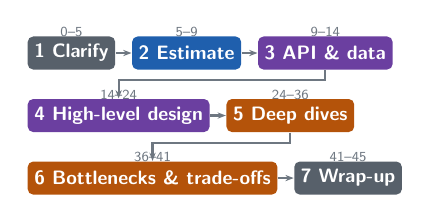
\begin{tikzpicture}[x=1cm,y=1cm,every node/.style={font=\scriptsize\bfseries,text=white,rounded corners=2pt,inner sep=2.4pt,minimum height=.42cm}]
  \node[fill=stA] (c) at (0,0) {1 Clarify};
  \node[fill=stB,right=.2 of c] (e) {2 Estimate};
  \node[fill=stC,right=.2 of e] (a) {3 API \& data};
  \node[fill=stC,below=.36 of c.south west,anchor=north west] (h) {4 High-level design};
  \node[fill=stD,right=.2 of h] (d) {5 Deep dives};
  \node[fill=stD,below=.36 of h.south west,anchor=north west] (b) {6 Bottlenecks \& trade-offs};
  \node[fill=stA,right=.2 of b] (w) {7 Wrap-up};
  \foreach \x/\y in {c/e,e/a,h/d,b/w} \draw[-{Stealth[length=3pt]},soft,thick] (\x) -- (\y);
  \draw[-{Stealth[length=3pt]},soft,thick] (a.south) |- ++(0,-.13) -| (h.north);
  \draw[-{Stealth[length=3pt]},soft,thick] (d.south) |- ++(0,-.13) -| (b.north);
  \foreach \n/\t in {c/0--5,e/5--9,a/9--14} \node[text=soft,font=\tiny,above=-.5pt of \n,fill=none,inner sep=0pt,minimum height=0pt] {\t};
  \foreach \n/\t in {h/14--24,d/24--36} \node[text=soft,font=\tiny,above=-.5pt of \n,fill=none,inner sep=0pt,minimum height=0pt] {\t};
  \foreach \n/\t in {b/36--41,w/41--45} \node[text=soft,font=\tiny,above=-.5pt of \n,fill=none,inner sep=0pt,minimum height=0pt] {\t};
\end{tikzpicture}
{\scriptsize\color{soft}\par Say the steps out loud at the start. Go broad before deep; every number must end in a decision.\par}

% ================================================================= clarify
\sect{stA}{\faClipboardList}{1 Clarify the requirements}{class 1 · $\approx$ 5 min}
\begin{bul}
  \item \term{Functional}: what it does (3--5 core features, and what you leave out). They decide the API and the data.
  \item \term{Non-functional}: how well. They decide the architecture. Each needs a \term{number, a percentile, a window and a load}: ``hold p99 $<$ 300 ms at 5\,000 holds/s''.
  \item Quality attributes: scalability, availability, latency, consistency, durability, cost, security, operability.
  \item \term{Scenario}: source $\to$ stimulus $\to$ environment $\to$ artifact $\to$ response $\to$ measure.
  \item Different data, different needs: seats and money strong; catalog 60 s stale; viewer counter approximate.
  \item If told ``you decide'', state an assumption: ``10 M daily users, reads:writes 100:1''.
\end{bul}
\begin{formula}{stA}
  \footnotesize\textbf{BoxOffice targets}: 2 M fans in the first minute for 60\,000 seats; normal peak 1\,500 catalog req/s. Catalog p99 $<$ 200 ms, hold p99 $<$ 300 ms, checkout p99 $<$ 1.5 s; checkout 99.95\%/30 days; 0 double bookings; RPO $=$ 0 for paid orders; $<$ R\$\,0.10 per ticket; MTTR $<$ 30 min.
\end{formula}
\trap{adjectives (``fast'', ``scalable'') instead of numbers; one target for everything; forgetting the peak.}

% ================================================================= estimate
\sect{stB}{\faCalculator}{2 Estimate}{class 2 · $\approx$ 4 min}
{\footnotesize Decision $\to$ assumptions $\to$ powers of ten $\to$ sanity check $\to$ conclusion. Within 2--3$\times$ is enough.\par}
{\footnotesize
\begin{tabularx}{\linewidth}{@{}l l X@{}}
  $2^{10}$ & $\approx 10^3$ & KB: a short JSON; 10 seat rows \\
  $2^{20}$ & $\approx 10^6$ & MB: a poster \\
  $2^{30}$ & $\approx 10^9$ & GB: RAM of a small VM \\
  $2^{40}$ & $\approx 10^{12}$ & TB: a large single-node database \\
  $2^{50}$ & $\approx 10^{15}$ & PB: a data lake \\
\end{tabularx}}
\begin{formula}{stB}
  \footnotesize 1 day $= 86\,400$ s $\approx 10^5$ s; 1 month $\approx 2.5\times10^6$ s; 1 year $\approx 3\times10^7$ s.\\
  1 M/day $\approx$ 12/s; 100 M/day $\approx$ 1\,200/s; 1 B/day $\approx$ 12\,000/s.\\
  1 Gbit/s $=$ 125 MB/s; 10 Gbit/s $=$ 1.25 GB/s (bits $\div$ 8).
\end{formula}
\begin{formula}{stB}
  $\text{QPS}_\text{avg} = \dfrac{\text{DAU} \times \text{actions/day}}{86\,400}$, \ peak $= 2$--$3\times$ avg\\[.15em]
  storage $=$ items/day $\times$ size $\times$ retention $\times$ replicas ($\times$1.5--2 indexes)\\
  bandwidth $=$ req/s $\times$ bytes per response
\end{formula}

\sub{stB}{Latency numbers (2020s, $\pm$ 2--3$\times$)}
{\footnotesize
\begin{tabularx}{\linewidth}{@{}X r@{}}
  L1 cache / main memory reference & 0.5 ns / 100 ns \\
  read 1 MB sequentially from memory & 10--50 µs \\
  NVMe SSD random 4 KB read & 10--100 µs \\
  read 1 MB sequentially from NVMe & 0.1--0.3 ms \\
  round trip inside an availability zone (AZ) & 0.1--0.5 ms \\
  Redis GET over the network, same AZ & 0.2--1 ms \\
  round trip between AZs of a region & 1--2 ms \\
  indexed PostgreSQL lookup, end to end & 1--5 ms \\
  HDD seek & 10 ms \\
  light in fibre, 1\,000 km one way & 5 ms \\
  São Paulo $\leftrightarrow$ US East round trip & 110--130 ms \\
  São Paulo $\leftrightarrow$ Western Europe & 180--220 ms \\
  TLS handshake on a new connection & $+$1--2 RTT \\
  LLM time to first token; then & 0.2--2 s; 30--150 tok/s \\
\end{tabularx}}
{\scriptsize\color{soft}Memory is $\approx$ 1\,000$\times$ faster than an SSD; a round trip in a data centre is $\approx$ 1\,000$\times$ faster than one across an ocean. 50 sequential calls of 0.5 ms $=$ 25 ms: batch them.\par}

\sub{stB}{Throughput of one instance (orders of magnitude)}
{\footnotesize
\begin{tabularx}{\linewidth}{@{}X r@{}}
  Nginx/Envoy, small responses & $10^4$--$10^5$ req/s \\
  app server, CRUD with one DB call & $10^2$--$10^4$ req/s \\
  PostgreSQL indexed reads / write tx & $10^4$--$10^5$ / $10^3$--$10^4$ \\
  Redis (single instance) & $\approx 10^5$ ops/s \\
  Kafka broker & $10^5$--$10^6$ msgs/s \\
  WebSocket server & $10^4$--$10^5$ connections \\
  DynamoDB partition & 3\,000 RCU / 1\,000 WCU \\
  S3 prefix & 3\,500 writes / 5\,500 reads/s \\
  Lambda per region (default) & 1\,000 concurrent \\
\end{tabularx}}

\sub{stB}{Sizes}
{\footnotesize UUID 16 B (36 as text) · timestamp 8 B · seat row $\approx$ 100 B · order or user row 0.5--1 KB · log line 0.2--2 KB · embedding 1\,536 float32 $\approx$ 6 KB · web page 50--200 KB · photo 0.2--3 MB · 1 min of 1080p video $\approx$ 38 MB.\par}

\sub{stB}{The on-sale on a napkin (BoxOffice)}
{\footnotesize
\begin{tabularx}{\linewidth}{@{}X r@{}}
  2 M fans refresh every $\approx$ 15 s & $\approx$ 130\,000 req/s \\
  behind a CDN with 99\% hits & $\approx$ 1\,300 req/s at origin \\
  edge bandwidth, 100 KB per view & $\approx$ 13 GB/s $\approx$ 100 Gbit/s \\
  hold attempts, 2 M in 60 s & $\approx$ 33\,000/s \\
  DB: $c = 8$ slots, $S = 5$ ms & 1\,600/s; 1\,100/s at 70\% \\
  waiting room admits & 1\,000 fans/s \\
  checkout sessions (Little) & 33/s $\times$ 5 min $\approx$ 10\,000 \\
  payments in flight & 17/s $\times$ 3 s $\approx$ 50 \\
  e-mails, 30\,000 tickets in 30 min & $\approx$ 17/s \\
\end{tabularx}}
\trap{designing for the average, false precision (``1\,157.4 req/s''), numbers without a conclusion.}

% ================================================================= queueing
\sect{stB}{\faStopwatch}{Load, latency and capacity}{classes 2 and 15}
\begin{formula}{stB}
  \textbf{Little}\quad $L = \lambda W$ \qquad \textbf{utilization}\quad $\rho = \dfrac{\lambda S}{c}$ \qquad $X_{\max} = \dfrac{c}{S}$\\[.1em]
  {\footnotesize $L$ in the system, $\lambda$ arrival rate, $W$ time in the system, $S$ service time, $c$ parallel slots. $1\,000/\text{s} \times 40$ ms $=$ 40 in flight; $8/5$ ms $=$ 1\,600/s.}
\end{formula}
\begin{formula}{stB}
  \textbf{M/M/1}\quad $R = \dfrac{S}{1 - \rho}$, \quad $\text{p99} \approx 4.6\,R$\\[.1em]
  {\footnotesize $S = 5$ ms: $\rho$ 50\% $\to$ 10 ms; 70\% $\to$ 17; 90\% $\to$ 50 (p99 230); 95\% $\to$ 100; 99\% $\to$ 500 ms. The knee: 70--80\% for one server; more servers move it right.}
\end{formula}
\begin{bul}
  \item Run latency-sensitive tiers at \term{50--70\%} at peak (batch 80--90\%): 4 replicas at 60\% lose one $\to$ 80\%; at 80\% $\to$ 107\%.
  \item \term{Closed} load test: $N = X\,(R + Z)$ (users, throughput, response, think time). 100 users, $R = 50$ ms $\to$ 2\,000 req/s; at 500 ms only 200. Real fans are an \term{open} model: arrivals do not wait.
  \item \term{Amdahl}: speedup $\le 1/\sigma$ (5\% serial $\to$ 20$\times$). \term{USL}: $C(N) = \frac{N}{1 + \sigma(N-1) + \kappa N(N-1)}$ peaks at $N^* = \sqrt{(1-\sigma)/\kappa}$, then falls.
\end{bul}
\begin{formula}{stB}
  $\text{replicas} = \left\lceil \dfrac{\text{peak}}{\text{capacity per replica} \times \rho_\text{target}} \right\rceil + \text{spares}$\\[.1em]
  {\footnotesize $4\,000 / (500 \times 0.65) \to 13$, $+1 = 14$. Plan with the knee, not the maximum, and add zone-loss replicas. Check shared resources: 500 DB connections $\div$ 20 per replica $=$ 25 replicas at most.}
\end{formula}

\sect{stB}{\faChartLine}{Percentiles and the tail}{classes 2 and 10}
\begin{formula}{stB}
  $P(\text{slow}) = 1 - (1 - q)^N$\quad {\footnotesize ($N$ calls in fan-out, each slow with probability $q$)}\\[.1em]
  {\footnotesize $q = 1\%$: $N = 5 \to 4.9\%$; $20 \to 18\%$; $100 \to 63\%$; $500 \to 99\%$.}
\end{formula}
\begin{bul}
  \item Percentiles come from \term{histograms}; never average them (p99s of 100 and 1\,000 ms are not 550). Sum the buckets, then compute.
  \item Tail tools: headroom, hedging after p95 (idempotent reads only), timeouts, partial results, warm pools.
\end{bul}
\trap{an 80 ms average can hide 5\% of fans waiting 4 s.}

% ================================================================= availability
\columnbreak
\sect{stD}{\faHeartbeat}{Availability, SLOs and error budgets}{classes 2, 9 and 10}
\begin{formula}{stD}
  $A = \dfrac{\text{MTTF}}{\text{MTTF} + \text{MTTR}}$ \quad series $\prod a_i$ \quad parallel $1 - \prod(1 - a_i)$\\[.1em]
  {\footnotesize 3 at 99.9\% in series $\to$ 99.7\%; 2 replicas at 99\% $\to$ 99.99\% (if independent); 2-of-3 quorum $= a^3 + 3a^2(1-a)$. MTTF 720 h, MTTR 2 h $\to$ 99.72\%; MTTR 2 min $\to$ 99.995\%: faster repair beats fewer failures.}
\end{formula}
{\footnotesize
\begin{tabularx}{\linewidth}{@{}l r r r r@{}}
  & \textcolor{soft}{year} & \textcolor{soft}{month} & \textcolor{soft}{28 days} & \textcolor{soft}{day} \\[-.1em]
  99\% & 3.65 d & 7.31 h & 6.72 h & 14.4 min \\
  99.9\% & 8.77 h & 43.8 min & 40.3 min & 1.44 min \\
  99.95\% & 4.38 h & 21.9 min & 20.2 min & 43.2 s \\
  99.99\% & 52.6 min & 4.38 min & 4.03 min & 8.64 s \\
  99.999\% & 5.26 min & 26.3 s & 24.2 s & 0.86 s \\
\end{tabularx}}
{\scriptsize\color{soft}Year $=$ 365.25 days, month $=$ 30.44 days. Always say the window. Rule of the extra nine: in a chain of $\approx$ 5 links, each link needs one nine more than the target.\par}
\begin{formula}{stD}
  SLI $= \dfrac{\text{good events}}{\text{valid events}}$ \quad error budget $= 1 - \text{SLO}$\\[.1em]
  burn rate $b = \dfrac{\text{observed error ratio}}{1 - \text{SLO}}$ \quad budget spent $= \dfrac{b \cdot t}{\text{window}}$\\[.1em]
  {\footnotesize 99.9\% over 28 days: 0.001 $\times$ 28 M requests $=$ 28\,000 failures, or 40.3 min. Burn 14.4 empties the 28-day budget in 1.9 days.}
\end{formula}
{\footnotesize
\begin{tabularx}{\linewidth}{@{}l c c c X@{}}
  & \textcolor{soft}{burn} & \textcolor{soft}{long} & \textcolor{soft}{short} & \textcolor{soft}{budget when it fires} \\[-.1em]
  page & 14.4$\times$ & 1 h & 5 min & 2\% \\
  page & 6$\times$ & 6 h & 30 min & 5\% \\
  ticket & 1$\times$ & 3 d & 6 h & 10\% \\
\end{tabularx}}
{\scriptsize\color{soft}Both windows must exceed the threshold: the short one makes the alert reset fast. Page on symptoms users feel, never on causes (CPU).\par}

% ================================================================= API & data
\sect{stC}{\faProjectDiagram}{3 API and data model}{classes 5 and 6 · $\approx$ 5 min}
\begin{bul}
  \item 4--6 endpoints for the core features: \texttt{GET /events}, \texttt{GET /events/\{id\}/seats}, \texttt{POST /holds}, \texttt{POST /orders} (with \texttt{Idempotency-Key}), \texttt{POST /payments/webhook}, \texttt{GET /orders/\{id\}}.
  \item \term{REST} for public resources; \term{gRPC} between services (HTTP/2, schemas); \term{GraphQL} for client-shaped reads (BFF); \term{async} (events) when nobody waits for the answer. Version without breaking shipped clients.
  \item Entities with their keys and access patterns: event, seat (status, version), hold (expires in 10 min), order (idempotency key), ticket.
  \item \term{SQL by default} for invariants and joins; \term{NoSQL} for huge write rates with simple key access; object store for blobs; search engine, warehouse and vector DB as derived copies.
\end{bul}
\begin{formula}{stC}
  \footnotesize\textbf{No double booking}: \texttt{UPDATE seat SET status='HELD' WHERE id IN (...) AND status='FREE'}; rows updated $\ne$ requested $\Rightarrow$ roll back, 409. A unique constraint is the last line of defence. A hot row caps throughput at $1/t$ (5 ms $\to$ 200/s).
\end{formula}
\trap{check-then-act (\texttt{SELECT}, then \texttt{UPDATE}) under read committed: two fans get seat A-12.}

\sub{stC}{Consistency, replication and partitioning}
\begin{formula}{stC}
  \textbf{Quorum}\quad $R + W > N$ \quad {\footnotesize ($N = 3$, $W = 2$, $R = 2$)}\quad \textbf{consensus}\quad $2f + 1$ nodes\\[.1em]
  {\footnotesize Read and write sets overlap, so a read sees the latest write. 3 nodes tolerate 1 failure, 5 tolerate 2; use odd $N$ spread so no zone holds a majority.}
\end{formula}
\begin{bul}
  \item Models, strong to weak: \term{linearizable} (seats, money) $\to$ sequential $\to$ causal $\to$ \term{read-your-writes} (a fan's own orders) $\to$ \term{eventual} (catalog, counters).
  \item \term{CAP}: during a partition choose consistency or availability. \term{PACELC}: else, choose latency or consistency, on every write ($\approx$ 1--2 ms across AZs, 150--200 ms across continents).
  \item \term{Replicas} scale reads, never writes, and lag (ms, seconds under load): read your own writes from the primary.
  \item \term{Partition} by a high-cardinality key read together (\texttt{event\_id, section}). \term{Consistent hashing} with virtual nodes moves $\approx 1/(N+1)$ of the keys when a node joins; \texttt{hash mod N} moves almost all.
  \item Across services: \term{sagas} with compensations and the \term{outbox}, not two-phase commit. Order comes from one authority or a per-key log, never from wall clocks of different machines.
\end{bul}
\trap{believing in exactly-once delivery: it is at-least-once $+$ idempotent processing.}

% ================================================================= high level
\sect{stC}{\faSitemap}{4 High-level design}{classes 4 to 8 · $\approx$ 10 min}
{\footnotesize Draw the happy path first, left to right, with the palette: client $\to$ DNS $\to$ CDN $\to$ WAF $\to$ load balancer / API gateway $\to$ stateless app servers $\to$ cache $\to$ SQL; the slow side branches go through a queue or a stream to workers; external providers behind adapters; observability on every box.\par}
\sub{stC}{Scale in steps: symptom $\to$ add $\to$ new problem}
{\footnotesize
\renewcommand{\arraystretch}{1.08}
\begin{tabularx}{\linewidth}{@{}>{\raggedright\arraybackslash}p{2.0cm}>{\raggedright\arraybackslash}X>{\raggedright\arraybackslash}p{2.1cm}@{}}
  one box fails all & separate SQL & a network hop \\
  CPU 85\% at peak & LB $+$ stateless replicas $+$ health check & sessions leave the server \\
  DB busy, 95\% reads & read replicas & lag, stale reads \\
  same 5 queries & cache & invalidation, stampede \\
  1 GB/s of images & CDN $+$ object store & edge invalidation \\
  checkout 2--3 s; spike & queue $+$ workers $+$ waiting room & duplicates, backlog \\
  5 teams, 1 codebase & services $+$ gateway $+$ events & network failures \\
  billions of rows & partitions $+$ search $+$ warehouse & hot partitions \\
  bots; region down & WAF, rate limits, multi-region & cross-region data \\
\end{tabularx}}
{\scriptsize\color{soft}Add a component only for a measured symptom. Monolith (modular) first.\par}

% ================================================================= deep dives
\columnbreak
\sect{stD}{\faSearchPlus}{5 Deep dives: the math of the hard parts}{$\approx$ 12 min}
\begin{formula}{stD}
  \textbf{Cache}\quad DB load $= (1 - h)\,\lambda$ \qquad $\bar t = h\,t_\text{hit} + (1 - h)\,t_\text{miss}$\\[.1em]
  {\footnotesize 50\,000 reads/s: $h$ 90\% $\to$ 5\,000 DB QPS; 99\% $\to$ 500; each nine is 10$\times$ less. TTL caps $h \le 1 - 1/(rT + 1)$ ($r$ reads/s of a key, $T$ TTL). Stampede $=$ reads/s $\times$ recompute time ($20\,000 \times 0.2$ s $=$ 4\,000 queries). Size for the working set: 20\,000 events $\times$ 4.1 KB $\approx$ 82 MB.}
\end{formula}
\begin{formula}{stD}
  \textbf{Queue}\quad backlog $= (\lambda - \mu)\,t$ \qquad wait $= \dfrac{\text{backlog}}{\mu}$ \qquad workers $= \lambda S$\\[.1em]
  {\footnotesize 6\,000/s against 2\,000/s for 3 min: 720\,000 waiting, the last waits 360 s. Drain $=$ backlog $\div$ (consume $-$ arrive). Divide by the drain rate, never the arrival rate.}
\end{formula}
\begin{formula}{stD}
  \textbf{Kafka}\quad partitions $\ge \max\!\left(\dfrac{T}{p}, \dfrac{T}{c}\right)$ \quad consumers per group $\le$ partitions\\[.1em]
  {\footnotesize $T$ target rate, $p$ and $c$ per-partition producer and consumer rates. 167 events/s, 20/s per consumer $\to$ $\ge$ 9 (choose 24). 6 partitions, 10 consumers $\to$ 4 idle. Order only per key.}
\end{formula}
\begin{formula}{stD}
  \textbf{Resilience}\quad in flight $= \lambda \times$ latency\\[.1em]
  {\footnotesize 100/s: 200 ms $\to$ 20 threads; 4 s $\to$ 400 $>$ 200: cascade. Timeout $\approx$ p99.9 (1.2 s $\to$ 2 s); 1 retry, backoff $\min(b\cdot 2^n, \text{cap})$ with full jitter; breaker 50\% of 20 calls, open 30 s; bulkhead 50. Retries at 3 layers: $3^3 = 27$ calls.}
\end{formula}
\begin{formula}{stD}
  \textbf{LLM}\quad cost $= \textstyle\sum_i (C_i\,p_\text{in} + O_i\,p_\text{out})$, \ $C_{i+1} = C_i + O_i + R_i$\\[.1em]
  {\footnotesize Context grows each step: input is $\approx$ quadratic in the steps. Latency $=$ TTFT $+$ TPOT$\,(N_\text{out} - 1)$: 0.6 s $+$ 20 ms $\times$ 249 $\approx$ 5.6 s. Agent success $p^n$: $0.95^{10} \approx 60\%$. KV cache 128 KiB/token: 8\,000 tokens $\approx$ 1 GiB.}
\end{formula}
\begin{formula}{stD}
  \textbf{Recovery}\quad RTO $\approx t_\text{detect} + t_\text{decide} + t_\text{promote} + t_\text{scale} + \text{TTL}$\\[.1em]
  {\footnotesize $2 + 5 + 1 + 5 + 1 \approx 14$ min. RPO: data lost, in time. Replicas copy a \texttt{DELETE} in ms: only backups with point-in-time recovery undo it. 2 TB at 200 MB/s $\approx$ 2.8 h to restore.}
\end{formula}

% ================================================================= bottlenecks
\columnbreak
\sect{stD}{\faStethoscope}{6 Bottlenecks: symptom $\to$ cause $\to$ what to do}{$\approx$ 5 min}
{\footnotesize
\renewcommand{\arraystretch}{1.1}
\begin{tabularx}{\linewidth}{@{}>{\raggedright\arraybackslash}p{2.15cm}>{\raggedright\arraybackslash}p{1.95cm}>{\raggedright\arraybackslash}X@{}}
  \textcolor{soft}{symptom} & \textcolor{soft}{cause} & \textcolor{soft}{what to do} \\[-.1em]
  p99 explodes, CPU idle, threads busy & slow dependency (Little) & timeout, breaker, bulkhead, async \\
  latency rises long before errors & past the knee ($\rho > 0.7$) & capacity, shed load, waiting room \\
  DB CPU high, mostly reads & no cache, low hit ratio & cache-aside, replicas, CDN \\
  DB spikes when a hot key expires & stampede & coalescing, TTL jitter, stale-while-revalidate \\
  one partition hot, the others idle & hot key & salt the key, cache it, admission control \\
  my update is not there & read from a lagging replica & read-your-writes from the primary \\
  consumer lag keeps growing & consumers $<$ load or $=$ partitions & more consumers, more partitions, faster handler \\
  duplicate e-mails or charges & at-least-once, no idempotency & idempotency key, dedupe in the same tx \\
  never recovers after a short outage & retry storm (metastable) & backoff $+$ jitter, retry budget, breaker \\
  errors for 30 s after a crash & no health check & readiness probes, short intervals \\
  minutes of errors after failover & DNS TTL, detection & lower TTL, faster checks, rehearse \\
  restarts everywhere on a DB blip & DB in the liveness probe & shallow liveness, local readiness \\
  429 at a burst (serverless) & concurrency limit, cold starts & raise limit, provisioned instances \\
  green dashboards, angry users & causes and averages & SLOs on percentiles, tracing \\
  LLM slow, 429, expensive & too many calls, long context & fewer steps, prefix cache, fallback, quotas \\
  invoice surprise & egress, NAT, logs & CDN, private endpoints, sampling \\
\end{tabularx}}

\sub{stD}{Trade-offs to say out loud}
\begin{bul}
  \item Cache: $-$latency and $-$DB load, $+$staleness (price up to 60 s old).
  \item Replicas: $+$reads, $+$lag. Sync replication: $+$durability, $+$write latency.
  \item Queue: $+$smooth load, $+$eventual consistency, duplicates.
  \item Strong consistency: correctness, at the cost of latency and availability in a partition.
  \item Second region: survives a region, $\approx 2\times$ the cost.
  \item Every quantified: ``adds $\approx$ 1 ms per request, cuts DB load 10$\times$''.
\end{bul}

% ================================================================= wrap-up
\columnbreak
\sect{stA}{\faFlagCheckered}{7 Wrap-up}{$\approx$ 3 min}
\begin{bul}
  \item Re-read the requirements and say how each is met, with its number.
  \item What you would measure: an SLO per journey, a burn-rate alert, one metric specific to the problem (hit ratio, consumer lag, replication lag).
  \item What fails first at 10$\times$, and what you would do next.
  \item What you left out on purpose.
\end{bul}
\trap{defending every decision as perfect: name the weakness before the interviewer does.}

\sect{stD}{\faLock}{Security and network in one breath}{class 11}
\begin{bul}
  \item VPC per region; subnets in $\ge$ 2 AZs: public (LB, NAT), private (apps), isolated (data). /16 $=$ 65\,536 addresses, /24 $=$ 256 (AWS reserves 5).
  \item \term{STRIDE} at every trust boundary: spoofing, tampering, repudiation, information disclosure, denial of service, elevation of privilege.
  \item OAuth 2.1: Authorization Code $+$ PKCE; access JWT $\approx$ 15 min, validated locally (revocation window $=$ lifetime).
  \item \term{Zero trust}: mTLS between services \emph{and} an authorization policy; authorize in the owning service (BOLA); secrets in a manager, rotated; signed images, SBOM.
\end{bul}
\trap{``the gateway validated the JWT, so we are safe'': authentication is not authorization.}

\sect{stC}{\faCloud}{Delivery and cost}{classes 12 and 14}
\begin{bul}
  \item Images small, immutable, by digest; probes local; requests sized; HPA: $\lceil \text{replicas} \times \text{current}/\text{target} \rceil$ ($\lceil 4 \times 90/60 \rceil = 6$). Autoscaling lags (pods 15 s steps, nodes minutes): pre-scale before 10:00.
  \item GitOps; canary 5\% $\to$ 25\% $\to$ 50\% $\to$ 100\% gated on error rate and p99 against the baseline; feature flags.
  \item Cost $=$ capacity $\times$ time. Data services, egress, logs and fixed hourly items (NAT, LB) dominate, not compute.
  \item AI in the pipeline: AI proposes, rules and humans decide. Precision beats recall; budgets live in the harness; judge by dollars per merged fix.
\end{bul}

\sect{stD}{\faBolt}{Measure it}{class 15}
\begin{bul}
  \item Profiles: smoke, load, stress, spike, soak, breakpoint. Open model for real traffic; watch \texttt{dropped\_iterations} $=$ 0.
  \item \term{Coordinated omission}: a closed test waits with the system and hides the queue (p99 1 ms vs 1\,366 ms).
  \item Find the bottleneck: RED (rate, errors, duration) per service $\to$ USE (utilization, saturation, errors) per resource $\to$ profile. Change one thing at a time.
\end{bul}


\columnbreak
\sect{stC}{\faSitemap}{BoxOffice on one page}{the reference design}
{\footnotesize The on-sale design that the classes build, drawn with the palette. Solid arrows: the fan waits; dashed: asynchronous.\par}
\vspace{.2em}
\begin{center}
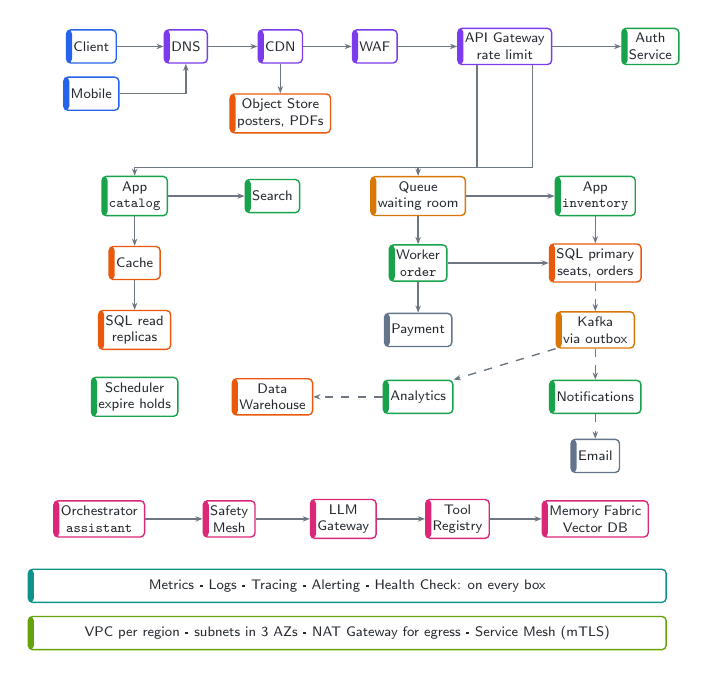
\begin{tikzpicture}[x=1cm,y=1cm,font=\sffamily\tiny,
  n/.style={draw=cat#1,line width=.5pt,fill=white,text=ink,rounded corners=1.5pt,inner xsep=2.5pt,inner ysep=1.8pt,minimum height=.42cm,align=center,
    path picture={\fill[cat#1] (path picture bounding box.south west) rectangle ([xshift=2pt]path picture bounding box.north west);}},
  a/.style={-{Stealth[length=2.6pt]},soft,line width=.5pt},
  d/.style={-{Stealth[length=2.6pt]},soft,line width=.5pt,dashed}]
  % clients and edge
  \node[n=client] (cl) at (0.45,0) {Client};
  \node[n=client] (mo) at (0.45,-.6) {Mobile};
  \node[n=edge] (dns) at (1.65,0) {DNS};
  \node[n=edge] (cdn) at (2.85,0) {CDN};
  \node[n=edge] (waf) at (4.05,0) {WAF};
  \node[n=edge] (gw) at (5.7,0) {API Gateway\\rate limit};
  \node[n=compute] (auth) at (7.55,0) {Auth\\Service};
  \node[n=storage] (obj) at (2.85,-.85) {Object Store\\posters, PDFs};
  \draw[a] (cl) -- (dns); \draw[a] (mo.east) -| (dns.south);
  \draw[a] (dns) -- (cdn); \draw[a] (cdn) -- (waf); \draw[a] (waf) -- (gw); \draw[a] (gw) -- (auth);
  \draw[a] (cdn) -- (obj);
  % read path (left)
  \node[n=compute] (cat) at (1.0,-1.9) {App\\\texttt{catalog}};
  \node[n=compute] (search) at (2.75,-1.9) {Search};
  \node[n=storage] (cache) at (1.0,-2.75) {Cache};
  \node[n=storage] (rep) at (1.0,-3.6) {SQL read\\replicas};
  \draw[a] (gw.south) ++(-.35,0) |- ++(0,-1.3) -| (cat.north);
  \draw[a] (cat) -- (search); \draw[a] (cat) -- (cache); \draw[a] (cache) -- (rep);
  % purchase path (middle and right)
  \node[n=messaging] (wr) at (4.6,-1.9) {Queue\\waiting room};
  \node[n=compute] (inv) at (6.85,-1.9) {App\\\texttt{inventory}};
  \node[n=compute] (ord) at (4.6,-2.75) {Worker\\\texttt{order}};
  \node[n=storage] (sql) at (6.85,-2.75) {SQL primary\\seats, orders};
  \node[n=external] (pay) at (4.6,-3.6) {Payment};
  \draw[a] (gw.south) ++(.35,0) |- ++(0,-1.3) -| (wr.north);
  \draw[a] (wr) -- (inv); \draw[a] (inv) -- (sql);
  \draw[a] (wr) -- (ord); \draw[a] (ord) -- (sql); \draw[a] (ord) -- (pay);
  % asynchronous side
  \node[n=messaging] (kaf) at (6.85,-3.6) {Kafka\\via outbox};
  \node[n=compute] (not) at (6.85,-4.45) {Notifications};
  \node[n=external] (mail) at (6.85,-5.2) {Email};
  \node[n=compute] (an) at (4.6,-4.45) {Analytics};
  \node[n=storage] (dwh) at (2.75,-4.45) {Data\\Warehouse};
  \node[n=compute] (sch) at (1.0,-4.45) {Scheduler\\expire holds};
  \draw[d] (sql) -- (kaf); \draw[d] (kaf) -- (not); \draw[d] (not) -- (mail);
  \draw[d] (kaf.south west) -- (an.north east); \draw[d] (an) -- (dwh);
  % AI
  \node[n=ai] (orc) at (0.55,-6.0) {Orchestrator\\\texttt{assistant}};
  \node[n=ai] (saf) at (2.2,-6.0) {Safety\\Mesh};
  \node[n=ai] (llm) at (3.65,-6.0) {LLM\\Gateway};
  \node[n=ai] (tool) at (5.1,-6.0) {Tool\\Registry};
  \node[n=ai] (mem) at (6.85,-6.0) {Memory Fabric\\Vector DB};
  \draw[a] (orc) -- (saf); \draw[a] (saf) -- (llm); \draw[a] (llm) -- (tool); \draw[a] (tool) -- (mem);
  % observability and network
  \node[n=observability,minimum width=8.1cm] (obs) at (3.7,-6.85) {Metrics · Logs · Tracing · Alerting · Health Check: on every box};
  \node[n=network,minimum width=8.1cm] (net) at (3.7,-7.45) {VPC per region · subnets in 3 AZs · NAT Gateway for egress · Service Mesh (mTLS)};
\end{tikzpicture}
\end{center}
{\scriptsize\color{soft}Read path: CDN, cache, replicas (eventual, seconds stale). Purchase: waiting room at the speed of the database and the provider; seats by conditional update in one primary (strong); payment with an idempotency key. Everything else is an event.\par}
\vspace{.4em}
\vspace{.3em}
\begin{alert}
  \textbf{Before you trust a design}: is every number tied to a decision? Is the peak (not the average) sized, with headroom for a lost node? Is every retry idempotent? Does every call have a timeout? Is strong consistency only where money and seats need it? What does the user see when each box fails?
\end{alert}

%%P3C3%%
\end{multicols*}


% ================================================================= pages 4 to 6: the palette
\newpage
\pagetitle{The palette, component by component}{The 44 components of the simulator: what, when, key numbers (``sim'': the playground default per replica), how it fails, products.}
\begin{multicols*}{3}
\cat{client}{Client}{who sends the traffic? · classes 1 and 4}
\begin{card}{client}{Client}{client}
\f{Is}{a browser, partner backend or load tester: you can neither patch nor trust it.}
\f{Use}{as the workload; what the user feels is DNS $+$ TLS $+$ round trips.}
\f{Numbers}{RTT São Paulo--US East $\approx$ 110--130 ms; nearby edge 5--20 ms; TLS 1.3 adds 1 RTT; ``instant'' $\approx$ 100 ms; 2 M fans in $\approx$ 1 min $\approx$ 33 k sessions/s.}
\ff{Fails}{retry storms (backoff + jitter, Retry-After); double submits (client idempotency key).}
\f{Products}{k6, Locust, Gatling; AWS/GCP/Azure SDKs; synthetic checks.}
\end{card}
\begin{card}{client}{Mobile}{mobile}
\f{Is}{a native or mobile-web app: flaky networks, battery, old versions, offline storage and push.}
\f{Use}{push, offline survival (QR ticket at the gate), a second traffic mix.}
\f{Numbers}{RTT 4G 30--100 ms, 3G 100--500 ms, 5G 10--30 ms; push in seconds, best effort.}
\ff{Fails}{drop mid-purchase (idempotency key + status endpoint); reconnect storms (jitter).}
\f{Products}{Firebase/FCM, APNs, Amplify, Notification Hubs.}
\end{card}

\cat{edge}{Traffic \& edge}{how does a request get in? · class 4}
\begin{card}{edge}{DNS}{dns}
\f{Is}{name $\to$ IP, cached for the TTL; managed DNS adds geo, weighted and failover routing; anycast.}
\f{Use}{always; the decision is the policy: region failover, latency/geo, weighted canary.}
\f{Numbers}{lookup cached 1--10 ms, full 20--120 ms; TTL 60--300 s for failover records. Failover $\approx$ interval $\times$ threshold $+$ TTL $= 3 \times 10 + 60$ s $\approx$ 1.5 min. Sim TTL 60 s.}
\ff{Fails}{provider outage (second provider); slow failover from cached answers.}
\f{Products}{Route 53 · Cloud DNS · Azure DNS · CoreDNS, BIND.}
\end{card}
\begin{card}{edge}{CDN}{cdn}
\f{Is}{edge caches (PoPs) near users; origin only on a miss; TLS and DDoS shield.}
\f{Use}{static assets and media, public read-heavy pages (event page with a TTL of seconds), video.}
\f{Numbers}{edge hit 5--30 ms vs 100+ ms to a far origin; static hit $>$ 90\%; origin $= (1-h) \times$ requests (95\% $\Rightarrow$ 1/20); egress 0.02--0.09 USD/GB. Sim $h = 0.9$.}
\ff{Fails}{cold cache or purge storm (versioned URLs, origin shield); caching private data.}
\f{Products}{CloudFront · Cloud CDN · Front Door · Cloudflare, Fastly, Varnish.}
\end{card}
\begin{card}{edge}{Load Balancer}{lb}
\f{Is}{spreads requests over healthy replicas; L4 (TCP) or L7 (HTTP: paths, TLS, retries).}
\f{Use}{as soon as there are two replicas: scale-out and zero-downtime deploys.}
\f{Numbers}{adds $<$ 1 ms; health check every 5--30 s, 2--3 failures to remove. Sim: detection 30 s without a Health Check, 3 s with one.}
\ff{Fails}{traffic to a dead replica until detected; a health check that lies (split liveness/readiness).}
\f{Products}{ALB/NLB · Cloud Load Balancing · Azure LB/App Gateway · HAProxy, Nginx, Envoy.}
\end{card}
\begin{card}{edge}{WAF}{waf}
\f{Is}{HTTP firewall: blocks SQLi, XSS and bots with managed + custom rules, at the edge.}
\f{Use}{in front of login, search and checkout; scalper bots; virtual patch; L7 DDoS.}
\f{Numbers}{adds $<$ 1 to a few ms; blocked requests never reach the origin. Sim blocks 95\% of bots.}
\ff{Fails}{false positives on real purchases; bypass by calling the origin directly.}
\f{Products}{AWS WAF · Cloud Armor · Azure WAF · ModSecurity + OWASP CRS.}
\end{card}
\begin{card}{edge}{API Gateway}{apigw}
\f{Is}{the API's front door: routing, JWT validation, rate limits, quotas. BFF: one per client type.}
\f{Use}{several services behind one API; per-user limits (429 + Retry-After); partner APIs.}
\f{Numbers}{adds 1--10 ms; Redis rate-limit check 0.5--1 ms. 429 = you are throttled, 503 = I am overloaded. Sim 10 k req/s.}
\ff{Fails}{the gateway is the bottleneck; no per-route timeouts; limiter store down (fail open or closed?).}
\f{Products}{API Gateway · Apigee · API Management · Spring Cloud Gateway, Kong.}
\end{card}
\begin{card}{edge}{Ingress}{ingress}
\f{Is}{Kubernetes rules for external HTTP(S) into Services, run by a controller; successor: Gateway API.}
\f{Use}{host/path routing, TLS with cert-manager, canary splits, GitOps routes.}
\f{Numbers}{adds $\le$ 1 ms; $\ge$ 2 controller replicas across zones; certificates 90 days, renewed.}
\ff{Fails}{under-provisioned controller; expired certificate; a rule shadowing a route.}
\f{Products}{AWS LB Controller · GKE Gateway · AGC · Traefik, Envoy Gateway.}
\end{card}

\cat{compute}{Compute}{where does the code run? · class 5}
\begin{card}{compute}{App Server}{app}
\f{Is}{stateless replicas running the business logic for requests a user waits on.}
\f{Use}{every synchronous API; modular monolith first; scale out behind an LB, autoscale at 50--70\% CPU.}
\f{Numbers}{limit $=$ threads $\div$ time per request: $200 \div 0.1$ s $=$ 2\,000 req/s. Sim 500 req/s, 10 ms, 120 USD/mo.}
\ff{Fails}{threads exhausted by a slow dependency (timeouts, breakers, bulkheads); past the knee as $\rho \to 1$.}
\f{Products}{EC2, ECS, EKS · Cloud Run, GKE · App Service, AKS · Spring Boot, FastAPI.}
\end{card}
\begin{card}{compute}{Worker}{worker}
\f{Is}{background processes pulling jobs from a queue or stream; the producer returns at once.}
\f{Use}{slow or unreliable work the user does not wait for (e-mail, PDF, transcoding); spike absorption.}
\f{Numbers}{workers $= \lambda \times$ job time: $500/\text{s} \times 0.2$ s $=$ 100; drain $=$ backlog $\div$ (consume $-$ produce): $600\text{k} \div 1\,000/\text{s} =$ 10 min. Sim 100 jobs/s, 50 ms.}
\ff{Fails}{poison message (max receives + DLQ); duplicates (dedupe table); hidden lag (alert on it).}
\f{Products}{Lambda + SQS · Cloud Run jobs · Functions + Service Bus · Celery, KEDA, Temporal.}
\end{card}
\begin{card}{compute}{Serverless}{serverless}
\f{Is}{functions run per event, scale from zero, billed per call and per GB-second.}
\f{Use}{spiky, short, event-driven work: webhooks, thumbnails, nightly jobs, glue.}
\f{Numbers}{cold start 0.1--1 s (JVM: seconds); Lambda 15 min max, 1\,000 concurrent per region (default). Instances $= \lambda \times W$. Sim cold start 600 ms.}
\ff{Fails}{throttling at the concurrency limit (429); connection storm on the DB (proxy/pooler).}
\f{Products}{Lambda · Cloud Run functions · Azure Functions · Knative, OpenFaaS.}
\end{card}
\begin{card}{compute}{Auth Service}{auth}
\f{Is}{authenticates users and issues short-lived JWT access tokens + refresh tokens (OAuth 2.1/OIDC).}
\f{Use}{any system with accounts; validate at the gateway, authorize in the services.}
\f{Numbers}{local JWT check $\approx$ µs; password hash $\ge$ 100 ms on purpose; access token 5--15 min.}
\ff{Fails}{auth down $=$ logged-in features down; login storm amplified by slow hashing.}
\f{Products}{Cognito · Identity Platform · Entra ID · Keycloak, ZITADEL.}
\end{card}
\begin{card}{compute}{Search}{search}
\f{Is}{ranked full-text, fuzzy and faceted queries over an inverted index; a secondary copy of the DB.}
\f{Use}{event search, autocomplete, facets; hybrid keyword + vector.}
\f{Numbers}{query 10--100 ms; refresh 1 s (near real time); autocomplete $<$ 100 ms end to end.}
\ff{Fails}{index out of sync (CDC/outbox + reconciliation); expensive queries; hot shards.}
\f{Products}{OpenSearch Service · Vertex AI Search · Azure AI Search · OpenSearch, Meilisearch.}
\end{card}
\begin{card}{compute}{Scheduler}{scheduler}
\f{Is}{triggers work by time (cron, delays) with one run guaranteed by a lock or leader.}
\f{Use}{release expired holds, reminders, opening the sale at 10:00, batch pipelines.}
\f{Numbers}{cron granularity 1 min; lock lease a few $\times$ job time. Sim: all jobs at once $=$ thundering herd.}
\ff{Fails}{double run (fencing token, idempotent jobs); missed run (dead-man's switch); herd at round hours (jitter).}
\f{Products}{EventBridge Scheduler · Cloud Scheduler · timer triggers · K8s CronJob, Quartz.}
\end{card}
\begin{card}{compute}{Notifications}{notifications}
\f{Is}{turns ``tell user X'' into push, e-mail or SMS: preferences, templates, dedupe, retries.}
\f{Use}{many services reaching users; isolation from provider quirks.}
\f{Numbers}{push in seconds; e-mail seconds to minutes; provider quotas per second and per day.}
\ff{Fails}{provider throttling (queue + backoff, second provider); duplicates; storms (kill switch).}
\f{Products}{SNS/SES · FCM · Notification Hubs · Novu.}
\end{card}
\begin{card}{compute}{Analytics}{analytics}
\f{Is}{events $\to$ stream $\to$ real-time counters and a warehouse for reports and funnels.}
\f{Use}{business metrics, A/B tests, live sale counters.}
\f{Numbers}{2 M fans $\times$ 20 events $\approx$ 40 M events in the sale hour; streaming seconds, batch hours; HyperLogLog 1--2\% error.}
\ff{Fails}{backlog delays dashboards; double counting under at-least-once.}
\f{Products}{Firehose, Redshift · BigQuery, Dataflow · Event Hubs · Kafka + Flink, ClickHouse.}
\end{card}

\cat{storage}{Storage}{where does the data live? · classes 6 and 7}
\begin{card}{storage}{SQL Database}{sql}
\f{Is}{tables, SQL and ACID transactions: the default system of record.}
\f{Use}{relations and invariants (``a seat is sold at most once''), joins, ad-hoc queries.}
\f{Numbers}{point read 0.1--1 ms (+ RTT); $10^3$--$10^4$ write tx/s; \texttt{max\_connections} 100; failover 30 s--min. Sim 3\,000 req/s.}
\ff{Fails}{connection exhaustion (PgBouncer); hot row in a flash sale (short tx, \texttt{SKIP LOCKED}, waiting room).}
\f{Products}{RDS, Aurora · Cloud SQL, AlloyDB, Spanner · Azure SQL · PostgreSQL, MySQL.}
\end{card}
\begin{card}{storage}{NoSQL DB}{nosql}
\f{Is}{key-value, document, wide-column or graph; partitioned by key and replicated.}
\f{Use}{very high write rates with simple key access: locations, chat, carts, timelines.}
\f{Numbers}{single-key op 1--10 ms; scales with partitions; DynamoDB 400 KB items, 3\,000 RCU/1\,000 WCU per partition; RF 3 ($W = R = 2$).}
\ff{Fails}{hot key (salt the key, cache it); stale reads under eventual consistency.}
\f{Products}{DynamoDB · Firestore, Bigtable · Cosmos DB · Cassandra, MongoDB.}
\end{card}

\begin{card}{storage}{Cache}{cache}
\f{Is}{in-memory copy of hot data, usually cache-aside with a TTL.}
\f{Use}{read-heavy, slow-changing data (catalog); expensive results; sessions and counters.}
\f{Numbers}{Redis GET 0.2--1 ms; $\approx 10^5$ ops/s per node; DB load $= (1-h) \times$ reads (90\% $\to$ 99\% $=$ 10$\times$ fewer); $\bar t = 0.95 \times 1 + 0.05 \times 20 \approx 2$ ms.}
\ff{Fails}{stampede on a hot key (coalescing, jittered TTL, stale-while-revalidate); cold cache after a flush.}
\f{Products}{ElastiCache, MemoryDB · Memorystore · Azure Managed Redis · Redis, Valkey, Memcached.}
\end{card}
\begin{card}{storage}{Object Store}{objstore}
\f{Is}{buckets of whole objects by key over HTTP: cheap, unlimited, very durable.}
\f{Use}{posters, PDF tickets, uploads, video, backups, data lake.}
\f{Numbers}{11 nines durability; first byte 10--100 ms; S3 3\,500 writes/5\,500 reads per s per prefix; $\approx$ 0.02 USD/GB-month.}
\ff{Fails}{public exposure (block public access); egress and tiny-request costs (CDN, lifecycle).}
\f{Products}{S3 · Cloud Storage · Blob Storage · MinIO, Ceph.}
\end{card}
\begin{card}{storage}{Data Warehouse}{dwh}
\f{Is}{columnar OLAP store for scans and aggregations over history, fed by ETL/ELT or CDC.}
\f{Use}{dashboards over months, joins of many sources, ML features.}
\f{Numbers}{seconds to minutes per query; compression 5--10$\times$; BigQuery $\approx$ 6 USD/TiB scanned.}
\ff{Fails}{analytics on the production DB; late pipelines (freshness alerts); runaway query cost.}
\f{Products}{Redshift, Athena · BigQuery · Fabric, Databricks · ClickHouse, Trino.}
\end{card}
\begin{card}{storage}{Vector DB}{vectordb}
\f{Is}{stores embeddings and answers approximate nearest-neighbour queries (HNSW, IVF).}
\f{Use}{RAG retrieval, semantic search, semantic cache, agent memory.}
\f{Numbers}{384--3\,072 dims; size $=$ dims $\times$ 4 B (1\,536 $\to$ 6 KB; 1 M $\to$ 6 GB); ANN 1--10 ms; recall@10 0.9--0.99.}
\ff{Fails}{right chunk not in top-$k$ (hybrid search, rerank); cross-tenant leakage (mandatory filters).}
\f{Products}{OpenSearch, pgvector · Vertex Vector Search · Azure AI Search · Qdrant, Milvus.}
\end{card}

\cat{messaging}{Messaging}{how do services talk without waiting? · class 8}
\begin{card}{messaging}{Message Queue}{queue}
\f{Is}{holds messages until one of several competing consumers acks them; failures go to a DLQ.}
\f{Use}{background jobs, spike absorption, load levelling (waiting room).}
\f{Numbers}{enqueue ms; drain $=$ backlog $\div$ (consume $-$ arrive): $120\text{k} \div 2\text{k/s} =$ 60 s; SQS visibility 30 s, retention 4 days (max 14).}
\ff{Fails}{poison message (max receives $\to$ DLQ); duplicates after a crash before the ack.}
\f{Products}{SQS · Cloud Tasks · Service Bus · RabbitMQ, BullMQ.}
\end{card}
\begin{card}{messaging}{Pub/Sub}{pubsub}
\f{Is}{publish once to a topic; every subscription gets a copy (each acts as its own queue).}
\f{Use}{fan-out of events (EventCancelled $\to$ refunds, notifications, search); chat delivery; cache invalidation.}
\f{Numbers}{publish-to-deliver tens of ms; 1 publish $\to N$ deliveries; GCP retention 7 days.}
\ff{Fails}{slow subscriber builds its own backlog; fire-and-forget loses messages.}
\f{Products}{SNS, EventBridge · Pub/Sub · Service Bus topics · NATS, Redis Pub/Sub.}
\end{card}
\begin{card}{messaging}{Event Stream}{stream}
\f{Is}{append-only, partitioned, retained log; each consumer group reads at its own offset and can replay.}
\f{Use}{many consumers of the same facts, CDC, event sourcing, ingestion.}
\f{Numbers}{Kinesis shard 1 MB/s or 1\,000 rec/s in; retention 24 h; parallelism per group $=$ partitions; watch consumer lag.}
\ff{Fails}{lag grows (more consumers, up to the partitions); lag beyond retention loses events.}
\f{Products}{Kinesis · Pub/Sub ordering keys · Event Hubs · Pulsar, NATS JetStream.}
\end{card}
\begin{card}{messaging}{Kafka}{kafka}
\f{Is}{topics of replicated partitions, consumer groups committing offsets, retention or compaction (KRaft).}
\f{Use}{event backbone, outbox + CDC (Debezium), high-volume pipelines with replay.}
\f{Numbers}{retention 7 days; RF 3, min ISR 2, \texttt{acks=all}; 6 partitions, 10 consumers $\Rightarrow$ 4 idle.}
\ff{Fails}{rebalance storms; poison message blocks a partition (retry + DLQ topics); duplicates before commit.}
\f{Products}{MSK · Managed Kafka · Event Hubs · Kafka, Strimzi, Confluent.}
\end{card}

\columnbreak
\cat{observability}{Observability}{how do we know? (side channels) · class 10}
\begin{card}{observability}{Metrics}{metrics}
\f{Is}{numeric time series with labels: counters, gauges, histograms. RED, USE, golden signals.}
\f{Use}{always: SLIs, SLOs, dashboards, alerts, autoscaling.}
\f{Numbers}{scrape 15--60 s; series $=$ metrics $\times$ label combos $\times$ instances ($50 \times 200 \times 20 =$ 200 k); 1--2 B/sample.}
\ff{Fails}{cardinality explosion; monitoring that dies with the system.}
\f{Products}{CloudWatch · Cloud Monitoring · Azure Monitor · Prometheus, Grafana.}
\end{card}
\begin{card}{observability}{Logs}{logs}
\f{Is}{timestamped event records, structured JSON with a \texttt{trace\_id}, in a central store.}
\f{Use}{investigating one request or user, errors with context, audit.}
\f{Numbers}{$2\,000 \text{ req/s} \times 5 \text{ lines} \times 500 \text{ B} = 5$ MB/s $\approx$ 430 GB/day; hot retention 7--30 days.}
\ff{Fails}{log flood in an incident (sample); no correlation id; secrets leaked.}
\f{Products}{CloudWatch Logs · Cloud Logging · Log Analytics · Loki, OpenSearch.}
\end{card}
\begin{card}{observability}{Tracing}{tracing}
\f{Is}{one request across services as a tree of spans under a trace id (W3C \texttt{traceparent}).}
\f{Use}{where latency or errors come from; retries, fan-out, agent runs.}
\f{Numbers}{tens to hundreds of spans per trace; head sampling 1--10\%; µs per span.}
\ff{Fails}{broken traces; sampling hides the rare slow request (tail sampling).}
\f{Products}{X-Ray · Cloud Trace · App Insights · OpenTelemetry, Jaeger, Tempo.}
\end{card}
\begin{card}{observability}{Alerting}{alerting}
\f{Is}{rules that page or ticket a human when users are affected: multi-window SLO burn rates.}
\f{Use}{every user-facing SLO; leading indicators (disk, certificates, lag near retention).}
\f{Numbers}{99.9\%/30 d $\approx$ 43 min; page at burn 14.4 over 1 h (2\% of the budget); $\le$ 2 incidents per shift.}
\ff{Fails}{alert fatigue; silent metric (absent-data alert, dead man's switch).}
\f{Products}{CloudWatch alarms · Cloud Monitoring · Azure Monitor · Alertmanager, Grafana.}
\end{card}
\begin{card}{observability}{Health Check}{healthcheck}
\f{Is}{probes deciding if an instance gets traffic (readiness) or is restarted (liveness); startup probe.}
\f{Use}{every replica behind an LB or Service; warm-up and shutdown; DNS failover.}
\f{Numbers}{detection $=$ interval $\times$ threshold (K8s $10 \times 3 \approx$ 30 s); lost requests $\approx$ share $\times$ detection.}
\ff{Fails}{restart storm; zombie returns 200 while requests fail (outlier detection).}
\f{Products}{ELB/Route 53 checks · GCLB checks · Azure probes · K8s probes, Actuator.}
\end{card}

\columnbreak
\cat{network}{Network}{who can talk to whom? · class 11}
\begin{card}{network}{VPC}{vpc}
\f{Is}{your isolated private network in one region; nothing in or out without gateways and routes.}
\f{Use}{always; one per environment; one per region for multi-region.}
\f{Numbers}{/16 $=$ 65\,536 IPs; RFC 1918: 10/8, 172.16/12, 192.168/16; RTT in an AZ 0.1--0.5 ms, between AZs 1--2 ms. Sim cross-region $+$70 ms.}
\ff{Fails}{overlapping CIDRs; everything in one AZ; open security group on the DB.}
\f{Products}{Amazon VPC · VPC network · VNet · Docker networks, kind.}
\end{card}
\begin{card}{network}{Subnet}{subnet}
\f{Is}{an address range in one AZ; public or private by its route table.}
\f{Use}{three tiers per AZ (public LB/NAT, private apps, isolated data), in $\ge$ 2 AZs.}
\f{Numbers}{/24 $=$ 256 addresses (AWS reserves 5 $\Rightarrow$ 251); cross-AZ $\approx$ 0.01 USD/GB each way; SGs stateful, NACLs stateless.}
\ff{Fails}{AZ outage; wrong route table (``private'' subnet with an IGW route).}
\f{Products}{VPC subnets + SGs · firewall rules · NSGs · NetworkPolicy (Cilium).}
\end{card}
\begin{card}{network}{NAT Gateway}{nat}
\f{Is}{outbound internet for private machines, unreachable from outside; lives in a public subnet.}
\f{Use}{private services calling payment, e-mail, LLM providers; fixed egress IPs for allow-lists.}
\f{Numbers}{$\approx$ 0.045 USD/h $+$ 0.045 USD/GB; up to 100 Gbps; sub-ms.}
\ff{Fails}{port exhaustion (keep-alive); zonal failure; per-GB cost surprise.}
\f{Products}{NAT Gateway · Cloud NAT · Azure NAT · iptables masquerade.}
\end{card}
\begin{card}{network}{VPN}{vpn}
\f{Is}{encrypted tunnel between networks (IPsec site-to-site, client VPN); interconnect for bandwidth.}
\f{Use}{hybrid systems (stadium DC $\to$ cloud), admin access.}
\f{Numbers}{$\le$ 1.25 Gbps per tunnel; adds 5--20 ms; 2 tunnels per connection; interconnect 1--100 Gbps.}
\ff{Fails}{tunnel down (two tunnels + BGP); MTU (MSS clamping); over-trust.}
\f{Products}{Site-to-Site VPN · HA VPN · VPN Gateway · WireGuard.}
\end{card}
\begin{card}{network}{Service Mesh}{mesh}
\f{Is}{a proxy per service (sidecar or ambient) $+$ control plane: mTLS, retries, splits, telemetry.}
\f{Use}{tens of services, zero trust in the cluster, canaries.}
\f{Numbers}{$\le$ 1 ms per hop at p50; sidecar tens of MB per pod; certs live hours.}
\ff{Fails}{retry amplification; control plane down blocks new pods.}
\f{Products}{VPC Lattice · Cloud Service Mesh · AKS Istio · Istio, Linkerd, Cilium.}
\end{card}

\cat{ai}{AI \& agents}{an LLM in production, safely · class 13}
\begin{card}{ai}{LLM Gateway}{llmgw}
\f{Is}{one proxy to every model provider: routing, fallbacks, quotas, budgets, caches, cost metrics.}
\f{Use}{several teams calling LLMs; outages and 429s; cost control.}
\f{Numbers}{TTFT 0.2--2 s; 30--150 tokens/s; semantic hit tens of ms. Sim quota 50 req/s, 1\,500 tokens, 0.003 USD/1k tokens.}
\ff{Fails}{provider outage or 429 (fallback, breaker); runaway cost (hard budgets).}
\f{Products}{Bedrock · Vertex AI · Azure AI Foundry · LiteLLM, Envoy AI Gateway.}
\end{card}
\begin{card}{ai}{Orchestrator}{orchestrator}
\f{Is}{runs the agent loop: model call $\to$ tool calls $\to$ repeat until an answer or a limit.}
\f{Use}{tasks needing data or actions the model lacks; paths that depend on results.}
\f{Numbers}{latency $\approx$ steps $\times$ per step ($6 \times 1.7$ s $\approx$ 10 s); cost $\approx$ steps $\times$ tokens $\times$ price; in flight $= 20/\text{s} \times 10 \text{ s} = 200$.}
\ff{Fails}{loops (step and token caps); partial execution (durable state, idempotency keys).}
\f{Products}{Bedrock Agents · Agent Engine · Foundry Agents · LangGraph, Temporal.}
\end{card}
\begin{card}{ai}{Tool Registry}{toolreg}
\f{Is}{the tools an agent may call: name, description, JSON schema, endpoint, permissions (MCP).}
\f{Use}{many tools, several agents, per-user authorization of calls.}
\f{Numbers}{5--20 tools per request; 50--300 tokens per definition; call 10--500 ms, timeout 1--5 s.}
\ff{Fails}{over-privileged tools (authorize with the user's identity); a slow tool stalls the agent.}
\f{Products}{AgentCore Gateway · Agent Builder · APIM as MCP · MCP servers.}
\end{card}
\begin{card}{ai}{Memory Fabric}{memory}
\f{Is}{context the model was not trained on: RAG (chunk, embed, retrieve, rerank), short- and long-term memory.}
\f{Use}{answers from your own changing data (refund policy), citations, personalization.}
\f{Numbers}{chunks 200--1\,000 tokens; top-$k$ 3--10; ANN 1--20 ms; rerank 50--300 ms.}
\ff{Fails}{retrieval miss; stale index; cross-tenant leak; memory poisoning.}
\f{Products}{Bedrock KB · RAG Engine · Azure AI Search · pgvector, LlamaIndex.}
\end{card}
\begin{card}{ai}{Safety Mesh}{safety}
\f{Is}{guardrails on input (injection, PII), output (moderation, grounding, schema) and actions.}
\f{Use}{any user-facing LLM feature; untrusted content; agents that act.}
\f{Numbers}{rules $<$ 1 ms; classifier 10--200 ms; LLM judge 0.5--2 s; eval set 50--200 examples. Sim catches 98\%.}
\ff{Fails}{indirect prompt injection; PII leak; hallucination; guardrail outage (fail open or closed?).}
\f{Products}{Bedrock Guardrails · Model Armor · Content Safety · NeMo Guardrails, Llama Guard.}
\end{card}

\cat{external}{External}{services we don't run · class 5}
\begin{card}{external}{3rd Party API}{thirdparty}
\f{Is}{someone else's API: a contract, a rate limit, a price, no access to their metrics.}
\f{Use}{buy, don't build, what is not your differentiator.}
\f{Numbers}{50--500 ms with a long tail; timeout a bit above p99 (p99 800 ms $\Rightarrow$ 1 s).}
\ff{Fails}{slow calls exhaust threads (timeout, breaker, bulkhead); 429 (backoff with Retry-After).}
\f{Products}{Resilience4j, Toxiproxy, WireMock; API Management as a proxy.}
\end{card}
\begin{card}{external}{Payment}{payment}
\f{Is}{a PSP: synchronous create/confirm (maybe ``pending'') $+$ a signed asynchronous webhook.}
\f{Use}{always for real money, behind an adapter (authorize, capture, refund, webhook).}
\f{Numbers}{authorization 0.5--3 s; webhooks late, twice or out of order; idempotency keys kept $\ge$ 24 h; seat hold 10 min.}
\ff{Fails}{double charge (one idempotency key per attempt); lost webhook (reconciliation).}
\f{Products}{Stripe, Adyen, Mercado Pago, PagBank, Pix PSPs; Hyperswitch.}
\end{card}
\begin{card}{external}{Email}{email}
\f{Is}{delivery provider with reputation-managed infrastructure and bounce webhooks.}
\f{Use}{transactional mail (ticket, receipt, reset), always via a queue.}
\f{Numbers}{60\,000 orders in 15 min $\approx$ 67 e-mails/s; $\approx$ 0.10 USD per 1\,000; bounces $<$ 2--5\%, complaints $<$ 0.1\%.}
\ff{Fails}{throttling (queue absorbs it); duplicates (key: order id $+$ template); spam folder.}
\f{Products}{SES · Communication Services · SendGrid, Postmark · Mailpit (dev).}
\end{card}

\cat{external}{Patterns that combine them}{classes 7 to 9, 13}
{\footnotesize
\renewcommand{\arraystretch}{1.06}
\sub{stC}{Caching (class 7)}
\begin{bul}
  \item \term{Cache-aside}: read cache, on a miss read DB and fill; on write, commit then \emph{delete} the key; TTL $+$ jitter as a safety net. Default.
  \item \term{Read-through} (a loader fills), \term{write-through} (cache and DB together), \term{write-behind} (DB later: may lose data), \term{refresh-ahead} (reload before expiry, e.g. at 80\% of the TTL).
  \item L1 in-process (1--5 s) $+$ Redis L2. Cache what you display, never what you decide on.
\end{bul}
\sub{stC}{Messaging (class 8)}
\begin{bul}
  \item \term{Load levelling}: a queue turns a spike into backlog (not a fix for a permanent shortage). \term{Waiting room}: admit at the measured rate of the bottleneck.
  \item \term{Transactional outbox}: write the event in the same transaction, relay later (or CDC); never dual writes.
  \item \term{Idempotent consumer}: dedupe table in the same transaction; bounded retries, then DLQ.
  \item \term{Saga}: local steps with compensations; the pivot (payment) is reconciled before compensating. Choreography for 2--3 steps, orchestration for 4$+$. \term{CQRS} and \term{event sourcing} only when a requirement asks.
\end{bul}
\sub{stD}{Resilience (class 9)}
\begin{bul}
  \item Timeout $\to$ one retry with backoff, jitter and an idempotency key $\to$ circuit breaker counting slow calls $\to$ bulkhead sized by Little $\to$ honest fallback (``seats held, payment pending'').
  \item \term{Load shedding} by priority protects the system; \term{rate limiting} protects it from one client (token bucket: capacity $=$ burst, rate $=$ sustained; 429 $+$ Retry-After).
\end{bul}
\sub{stC}{AI (class 13)}
\begin{bul}
  \item Workflow first, agent where needed (capped steps); gateway with fallbacks, token quotas, prefix caching; RAG with hybrid search, rerank, citations; live data through tools; least privilege and UI confirmation for irreversible actions.
\end{bul}}

\end{multicols*}


% ================================================================= pages 7 and 8: class by class
\newpage
\pagetitle{Class by class}{Each class's question, what to take away and its most common trap. The pages: insper.github.io/platform/2027.1/classes/.}
\begin{multicols*}{3}
\begin{klass}{}{1 · What is System Design}{intro · clarify}
\question{2 M fans hit 60\,000 seats at 10:00: which decisions above the code decide whether BoxOffice answers in time and sells each seat once?}
\begin{light}
  \item Requirements drive design: functional decide API and data; non-functional (number, percentile, window, load) decide the architecture.
  \item Architectures evolve: add a component for a measured symptom and expect the new problem it brings.
  \item Seven time-boxed steps: clarify, estimate, API and data, high level, deep dives, bottlenecks, wrap-up.
\end{light}
\nums{hold p99 $<$ 300 ms, checkout p99 $<$ 1.5 s, 99.95\%/28 days, catalog 60 s stale; interview minutes 5 · 4 · 5 · 10 · 12 · 5 · 3.}
\say{Before I draw, let me agree on the requirements and do a quick estimate.}
\pit{jumping to technology names before requirements and numbers.}
\end{klass}

\begin{klass}{}{2 · Estimation \& Performance Math}{estimation · estimate}
\question{Can one PostgreSQL take the on-sale? Requests per second, time per hold, safe utilization, the slow call behind a page.}
\begin{light}
  \item Estimate to pick a side of a threshold: 33\,000 holds/s against $8/5\text{ ms} = 1\,600$/s $\Rightarrow$ waiting room at 1\,000/s.
  \item $L = \lambda W$, $X_{\max} = c/S$, $R = S/(1-\rho)$: run at 50--70\%.
  \item Users feel percentiles and chains: $1-(1-q)^N$, $\prod a_i$.
\end{light}
\nums{1 day $\approx 10^5$ s; 1 M/day $\approx$ 12/s; AZ round trip 0.5 ms; São Paulo--Virginia 120 ms; at 90\% $R = 10\,S$.}
\say{About 400 reads/s, 1\,200 at peak: one server and a cache.}
\pit{sizing for the average (load, latency, availability of one box) instead of peak, tail and chain.}
\end{klass}

\begin{klass}{}{3 · Distributed Systems}{distributed · design}
\question{A ``Hold seat'' times out after 5 s and the fan presses again: is she holding two seats? Will she pay twice?}
\begin{light}
  \item A timeout cannot tell slow from dead: every retried operation must be idempotent (conditional write or idempotency key).
  \item Consistency per data: linearizable (majority, $R + W > N$) for seats and money; read-your-writes for a fan's data; eventual for the catalog.
  \item Majorities overlap: odd $N$ across zones; leases need fencing tokens; sagas and outbox across services, not 2PC.
\end{light}
\nums{$R + W > N$ (3, 2, 2); $2f + 1$ nodes; a write pays 1--2 ms across AZs, 150--200 ms across continents.}
\say{Seats are linearizable through one leader; the catalog is eventually consistent.}
\pit{believing in exactly-once delivery, or ordering events by the wall clocks of different machines.}
\end{klass}

\begin{klass}{}{4 · Traffic \& Edge}{edge · design}
\question{2 M fans press refresh at 10:00:00: which hops absorb, filter and route the traffic so only a fair, healthy stream reaches \texttt{inventory}?}
\begin{light}
  \item Each hop removes load from the next: origin $=$ traffic $\times$ miss rate (200 k req/s at 99\% $\to$ 2 k).
  \item Token bucket: capacity $=$ burst, rate $=$ sustained; shared atomic counters across replicas; 429 $+$ Retry-After.
  \item Latency is round trips $\times$ distance: reuse connections, terminate near the user; consistent hashing moves $1/(N+1)$ of keys.
\end{light}
\nums{DNS failover $\approx 3 \times 10 + 60$ s; new connection: TCP $+$ TLS 2--3 RTT, QUIC 1; fan limit 10 req/s, burst 20.}
\say{Everything identical for every fan comes from the CDN; the origin sees only the misses.}
\pit{thinking in hit ratio, not miss rate (95\% $\to$ 99\% is 5$\times$ less origin load); believing DNS failover is fast.}
\end{klass}

\begin{klass}{}{5 · Compute \& Services}{compute · design, estimate}
\question{Millions of page views, seats held without double booking, cards charged, 60\,000 tickets: and a few hundred req/s at 03:00. Where does each piece of work run?}
\begin{light}
  \item Stateless tier: $\lceil \text{peak}/(\text{cap} \times \rho) \rceil +$ spare ($4\,000/(500 \times 0.65) \to 13 + 1$).
  \item Little everywhere: workers $= \lambda \times$ job time; Lambda concurrency $=$ rate $\times$ duration.
  \item Integrations: idempotency keys from the logical operation, timeout $=$ unknown, signed deduplicated webhooks, reconciliation.
\end{light}
\nums{200 threads $\div$ 0.1 s $=$ 2\,000 req/s; cold start 0.1--1 s; 500 DB connections $\div$ 20 $=$ 25 replicas; hold 10 min.}
\say{The purchase answers 202; the e-mail and the PDF follow from a queue.}
\pit{assuming elasticity and duplication are free: autoscaling takes minutes; cron and retries run $N$ times.}
\end{klass}

\begin{klass}{}{6 · Databases \& Data Systems}{databases · design}
\question{One PostgreSQL holds everything; at 10:02 CPU is 100\%, a report locks for 40 s and seat A-12 is sold twice. What goes where?}
\begin{light}
  \item Choose by access pattern, volume and consistency: relational for invariants; 60\,000 seats is tiny, contention is the hard part.
  \item Put the check inside the write (conditional \texttt{UPDATE}, rowcount 1, unique constraint); a hot row caps at $1/t$.
  \item Replicas scale reads and lag; partition by a high-cardinality key with consistent hashing; expect the hot partition.
\end{light}
\nums{hot row 5 ms $\Rightarrow$ 200/s; consistent hashing moves $\approx 1/N$ of keys, \texttt{mod N} $\approx$ 90\%; B-tree fan-out $\approx$ 500.}
\say{Seats live in PostgreSQL behind a conditional update; I shard only when writes force me to.}
\pit{check-then-act under read committed; reading your own write from an async replica.}
\end{klass}

\begin{klass}{}{7 · Caching}{caching · design, deep dive}
\question{Tens of thousands of \texttt{GET /events/42} per second run the same three queries on data unchanged for a week: how do we serve a copy without acting on a stale one?}
\begin{light}
  \item Think in miss ratio: DB QPS $= (1-h)\lambda$; each nine is 10$\times$ less load.
  \item Cache-aside: write DB, commit, then delete the key; TTL with jitter; cache what you display, not what you decide on.
  \item Once the DB is sized for misses, the cache is load-bearing: stampede $=$ reads/s $\times$ recompute time; L1 for hot keys.
\end{light}
\nums{50\,000 reads/s: $h$ 90\% $\to$ 5\,000 DB QPS, 99\% $\to$ 500; Redis 0.2--1 ms, $\approx 10^5$ ops/s; stampede $20\,000 \times 0.2 = 4\,000$.}
\say{Cache-aside, TTL 5 min with jitter, delete after commit, 2-second L1.}
\pit{treating 95\% $\to$ 99\% as ``4 points'' (it is 5$\times$ fewer misses); deleting the key before the commit.}
\end{klass}

\begin{klass}{}{8 · Messaging \& Event-Driven}{messaging · design, deep dive}
\question{The e-mail provider goes from 80 to 800 ms and purchases fail: which steps must the fan wait for, and how do we hand off the rest safely?}
\begin{light}
  \item Go async for work nobody waits for: the chain availability becomes order $\times$ broker (99.65\% $\to$ 99.90\%).
  \item Queue math: backlog $= (\lambda-\mu)t$, wait $=$ backlog$/\mu$, partitions $\ge T/c$, consumers $\le$ partitions.
  \item At-least-once: idempotent consumers, bounded retries $+$ DLQ, outbox instead of dual writes, sagas with a payment pivot.
\end{light}
\nums{6\,000 vs 2\,000/s for 3 min $\to$ 720\,000 waiting, 360 s; RF 3, \texttt{acks=all}, min ISR 2; retention 7 days.}
\say{Order events keyed by order id, idempotent consumers, and I alert on consumer lag.}
\pit{dividing the backlog by the arrival rate; trusting exactly-once; dual writes.}
\end{klass}

\begin{klass}{}{9 · Reliability \& Resilience}{reliability · deep dive}
\question{The payment provider goes from 200 ms to 4 s and nothing is broken: how do we stop it taking down \texttt{order}, the gateway and browsing, and how much failure is acceptable?}
\begin{light}
  \item Availability is arithmetic: lower MTTR beats higher MTTF; series multiplies; the unreplicated part dominates.
  \item SLO $\to$ error budget $\to$ burn rate turns ``reliable enough?'' into decisions: ship or freeze, page or ticket.
  \item Slow is worse than dead: timeout, one jittered retry, breaker on slow calls, bulkhead by Little, honest fallback.
\end{light}
\nums{720 h / 2 h $\to$ 99.72\%; burn 14.4 over 1 h $\approx$ 2\% of the budget; breaker 50\% of 20 calls, open 30 s; bulkhead 50.}
\say{Payment gets a 2 s timeout, one jittered retry with an idempotency key, a breaker and a bulkhead.}
\pit{retries at every layer (27$\times$) and replicas as backups (they copy the \texttt{DELETE}).}
\end{klass}

\begin{klass}{}{10 · Observability}{observability · deep dive}
\question{Every pod is green, CPU 45\%, errors 0.3\%, yet the median fan waits 9 s to pay. What would have found the slow hop in minutes?}
\begin{light}
  \item Measure what users feel per journey: percentiles and SLIs; multiwindow burn-rate alerts (14.4$\times$ 1 h/5 min).
  \item Shared context (\texttt{trace\_id}, exemplars, \texttt{traceparent}) turns signals into one investigation: 7.9 s in \texttt{pool.acquire}.
  \item Telemetry costs: bound cardinality, tail-sample traces (7.8\% kept, 100\% of errors). Mitigate first; blameless postmortems.
\end{light}
\nums{series $=$ metrics $\times$ label values $\times$ instances (204\,000; $\times 10^6$ with \texttt{customer\_id}); traces $500 \times 8 \times 500$ B $=$ 2 MB/s.}
\say{Metrics to detect, traces to locate, logs to explain.}
\pit{green dashboards of causes and averages; averaging per-pod p99s (450 vs 756 ms).}
\end{klass}

\begin{klass}{}{11 · Network \& Security}{network-security · design}
\question{Who can talk to whom, and how does each call prove who it is and what it may do, from the fan's phone to \texttt{payment}?}
\begin{light}
  \item Security is a design decision: STRIDE at every trust boundary, independent layers.
  \item Isolation from routes, security groups and NetworkPolicy; a NAT per AZ; endpoints for cloud services; plan CIDRs.
  \item Identity everywhere, short-lived: Authorization Code $+$ PKCE, 15-min JWTs, mTLS $+$ authorization policy, rotated secrets, verified signatures.
\end{light}
\nums{/16 $=$ 65\,536, /24 $=$ 256 (5 reserved); access token 15 min; NAT $\approx$ 0.045 USD/h $+$ 0.045 USD/GB.}
\say{Only the load balancer is public; the database subnet has no route to the internet.}
\pit{authentication taken for authorization (BOLA); STRICT mTLS without an authorization policy.}
\end{klass}

\begin{klass}{}{12 · Cloud-Native Platforms}{cloud-native · design, estimate}
\question{From one \texttt{docker compose up} to 20$\times$ traffic for 30 minutes, a fix at 09:55 without downtime, and the cost known before the invoice.}
\begin{light}
  \item Stateless, disposable apps in small immutable images; graceful shutdown.
  \item Kubernetes reconciles desired state: right requests, local probes, HPA $\lceil 4 \times 90/60 \rceil = 6$; pre-scale before 10:00.
  \item GitOps and canaries gated on error rate and p99; cost $=$ capacity $\times$ time (CDN, data, egress dominate).
\end{light}
\nums{HPA $\lceil 4 \times 90/60 \rceil = 6$; canary 5 $\to$ 25 $\to$ 50\%, gate errors $<$ 0.5\%, p99 $<$ 300 ms; $\approx$ 0.013 USD per ticket.}
\say{We pre-scale at 09:45: the autoscaler reacts in minutes, the on-sale in seconds.}
\pit{the database in readiness or liveness probes; ``the HPA will save the on-sale''.}
\end{klass}

\begin{klass}{}{13 · AI Systems \& Agents}{ai-systems · design, estimate}
\question{``Find two seats under R\$\,300 and hold them'': answered in seconds, within rate limits and budget, without invented holds or obeying text hidden in a venue page?}
\begin{light}
  \item The LLM is a capacity-bound dependency: cost and latency $\approx$ calls $\times$ tokens; context grows each step (4 $\to$ 10 calls: cost 3.6$\times$).
  \item The model proposes tools; the orchestrator decides (as the user, budgets, idempotency, risk tiers). Knowledge via RAG, live data via tools.
  \item Safety is architectural; quality needs evals (golden set, pass$^k$) and GenAI traces.
\end{light}
\nums{4 calls $\approx$ 17\,000 input tokens; $0.95^{10} \approx 60\%$; latency $=$ TTFT $+$ TPOT$(N-1)$; KV cache 128 KiB per token.}
\say{Five components, not one LLM box: gateway, orchestrator, tools, memory, safety.}
\pit{prompt caching (safe) confused with semantic caching (false hits); reporting pass@k.}
\end{klass}

\begin{klass}{}{14 · AI-Assisted Delivery}{ai-delivery · deep dive}
\question{12 engineers, 60 PRs a week: where should AI steps sit in the pipeline to cut review latency without noise, deleted tests or surprise invoices?}
\begin{light}
  \item Each AI step has a contract: trigger, untrusted context, validated output, least-privilege action, budget, fail direction.
  \item Tokens are cents; attention is the cost: precision beats recall (41\% at 3 comments per PR is ignored).
  \item Judge deterministically: mutation score, external verification, statistical canary verdicts; agent cost is quadratic in turns.
\end{light}
\nums{review $\approx$ 0.02--0.09 USD; 40\% precision $\times$ 4 comments $\times$ 5\,000 reviews/week $\approx$ 12\,000 useless; 10 $\to$ 40 turns: 1.33 $\to$ 11.32 USD.}
\say{AI proposes; rules and humans dispose.}
\pit{letting the model decide (approve, merge, quarantine, roll back) or trusting instructions in the prompt.}
\end{klass}

\begin{klass}{}{15 · Performance Engineering}{performance · estimate, deep dive}
\question{Last year's on-sale fell at 10:02 after an ``all green'' test of 200 virtual users. How do you test so it does not happen again?}
\begin{light}
  \item $R = S +$ waiting; $N = XR$ and $U = XS$ tie the numbers; latency explodes near saturation.
  \item Plan with the knee, not the maximum: replicas $= \lceil \text{peak}/(\text{knee} \times (1 - \text{headroom}))\rceil$ $+$ zone loss.
  \item Open model, realistic data, per-endpoint thresholds; RED $\to$ USE $\to$ profile; one change at a time.
\end{light}
\nums{closed model backs off 182 $\to$ 67 req/s; peak 4\,500 holds/s, 275 per pod at the knee $\to$ 22 pods, 33 with a zone loss.}
\say{We test with an open model and require zero dropped iterations.}
\pit{a closed-model test against open-world traffic (coordinated omission: p99 1 ms vs 1\,366 ms).}
\end{klass}

\begin{klass}{}{16 · Case Studies}{case-studies · all stages}
\question{URL shortener, rate limiter, feed, chat, rides, video, notifications, payments, autocomplete, ticketing, AI assistant, cache: how do you solve any of them in 45 minutes?}
\begin{light}
  \item Follow the framework in order and end every estimate in a decision (``hot set 33 GB fits in memory $\Rightarrow$ cache'').
  \item Twelve cases, eight patterns; Little's Law and the hit-ratio formula appear in almost every estimate.
  \item Correctness lives in idempotency and atomic guards; strong consistency only for seats, money and assignment.
\end{light}
\nums{7 base62 characters $=$ 3.5 trillion codes; in flight $=$ rate $\times$ latency; DB load $= (1-h)\lambda$.}
\say{Let me clarify, estimate and then draw; every number ends in a decision.}
\pit{rate limiting or autoscaling a resource that cannot scale (hot row, primary, PSP limit): it needs admission control.}
\end{klass}
\vspace{.2em}
\sub{sim}{\faMousePointer\ The 25 playground scenarios}
{\scriptsize\renewcommand{\arraystretch}{1.0}
\begin{tabularx}{\linewidth}{@{}>{\ttfamily}l X@{}}
monolith & the first box to saturate sets the breaking point \\
scale-out & N$+$1 replicas; health checks detect the dead one \\
read-heavy-cache & DB load $= (1-h)\times$ reads; flush $\to$ stampede \\
cdn-static & static bytes stay at the edge \\
db-replicas & replicas add reads, not writes, and lag \\
sharding & partitions scale until one key is hot \\
async-queue & a queue turns a spike into backlog \\
event-fanout & each consumer group reads at its own pace \\
cascading-failure & slow dependency $\to$ threads exhausted (Little) \\
retry-storm & retries without backoff never let it recover \\
rate-limiter & reject the excess fast (429) \\
multi-region & failover $=$ detection $+$ DNS TTL \\
serverless-burst & cold starts and concurrency limits \\
flash-sale & CDN, cache and a waiting room for the peak \\
url-shortener & key lookup, read-heavy \\
news-feed & fan-out on write vs on read \\
chat & store partitioned, deliver by pub/sub \\
ride-sharing & a write-heavy geo index \\
video-streaming & CDN $+$ object store $+$ transcoding workers \\
notification-system & queue in front of provider quotas \\
payment-system & retries need idempotency keys \\
search-autocomplete & a latency budget met by a cache \\
ai-assistant & LLM calls set latency and cost \\
observability-stack & you can't fix what you don't measure \\
blank & an empty canvas for your own design \\
\end{tabularx}}
{\scriptsize\color{soft}insper.github.io/platform/playground/scenarios/\#\textless id\textgreater\par}
\vspace{.3em}
{\scriptsize\color{soft}Design adapted from the instructor's Machine Learning cheat sheet. Colours: grey clarify, blue estimate, purple design, orange deep dive, green answer, red trap; chips: simulator categories.\par}
\end{multicols*}


\end{document}
